
%%--------------------------------------------------
%% CPO: Multiple Choice Questions
%%--------------------------------------------------


%% Chapter 15: Electrical Charges and Forces
%%--------------------------------------------------


%% Learning Objectives
%%--------------------------------------------------

%% Distinguish between a positive and negative net charge. 
%% Explain the meaning of Coulomb’s law. 
%% Describe different ways of charging an electroscope.
%% Describe the relationship between electrons and current. 
%% Explain, at the atomic level, the difference between insulators, semiconductors, and conductors.
%% Identify how voltage and charge are related.  
%% Describe what happens in a capacitor as it charges. 
%% Recognize that current decreases over time as a capacitor charges or discharges. 
%% Explain the factors that determine how much charge a capacitor holds.


%% CPO Multiple Choice Questions
%%--------------------------------------------------
\element{cpo-mc}{
\begin{question}{cpo-ch15-q01}
    A device used to observe electric forces is a(n):
    \begin{multicols}{2}
    \begin{choices}
        \wrongchoice{galvanometer}
        \wrongchoice{voltmeter}
        \wrongchoice{compass}
      \correctchoice{electroscope}
    \end{choices}
    \end{multicols}
\end{question}
}

\element{cpo-mc}{
\begin{question}{cpo-ch15-q02}
    The unit of charge is the:
    \begin{multicols}{2}
    \begin{choices}
        \wrongchoice{ohm (\si{\ohm})}
        \wrongchoice{ampere (\si{\ampere})}
        \wrongchoice{volt (\si{\volt})}
      \correctchoice{coulomb (\si{\coulomb})}
    \end{choices}
    \end{multicols}
\end{question}
}

\element{cpo-mc}{
\begin{question}{cpo-ch15-q03}
    The negatively charged particle in an atom is a(n):
    \begin{multicols}{2}
    \begin{choices}
      \correctchoice{electron}
        \wrongchoice{proton}
        \wrongchoice{neutron}
        \wrongchoice{neutrino}
    \end{choices}
    \end{multicols}
\end{question}
}

\element{cpo-mc}{
\begin{question}{cpo-ch15-q04}
    An object with equal amounts of positive and negative charge is called:
    \begin{choices}
        \wrongchoice{positively charged}
        \wrongchoice{negatively charged}
      \correctchoice{neutral}
        \wrongchoice{electrically charged}
    \end{choices}
\end{question}
}

\element{cpo-mc}{
\begin{question}{cpo-ch15-q05}
    Positive electric charges:
    \begin{choices}
        \wrongchoice{attract both positive charges and negative charges.}
        \wrongchoice{repel both positive charges and negative charges.}
        \wrongchoice{attract positive charges and repel negative charges.}
      \correctchoice{repel positive charges and attract negative charges.}
    \end{choices}
\end{question}
}

\element{cpo-mc}{
\begin{question}{cpo-ch15-q06}
    Electric charge is:
    \begin{choices}
        \wrongchoice{caused by two fluids, as described by Benjamin Franklin.}
        \wrongchoice{present in metals only.}
      \correctchoice{a fundamental property of matter that has two types, positive and negative.}
        \wrongchoice{found only in non-living material.}
    \end{choices}
\end{question}
}

\element{cpo-mc}{
\begin{question}{cpo-ch15-q07}
    The buildup of static charge on an object is called:
    \begin{choices}
        \wrongchoice{inductive electricity.}
      \correctchoice{static electricity.}
        \wrongchoice{contact electricity.}
        \wrongchoice{charged electricity.}
    \end{choices}
\end{question}
}

\element{cpo-mc}{
\begin{question}{cpo-ch15-q08}
    One ampere is defined as:
    \begin{choices}
        \wrongchoice{a difference of one volt per second.}
      \correctchoice{the flow of one coulomb per second.}
        \wrongchoice{the resistance of one ohm per second.}
        \wrongchoice{the capacity of one farad per second.}
    \end{choices}
\end{question}
}

\element{cpo-mc}{
\begin{question}{cpo-ch15-q09}
    The charge of a proton and the charge of an electron have:
    \begin{choices}
        \wrongchoice{different amount of charge and opposite sign.}
      \correctchoice{the same amount of charge and opposite sign.}
        \wrongchoice{different amount of charge and the same sign.}
        \wrongchoice{the same amount of charge and the same sign.}
    \end{choices}
\end{question}
}

\element{cpo-mc}{
\begin{question}{cpo-ch15-q10}
    The diagram that best represents the charge distribution on a neutral electroscope when a negatively charged rod is held near it is:
    \begin{multicols}{2}
    \begin{choices}
        \AMCboxDimensions{down=-1.5cm}
        \wrongchoice{
            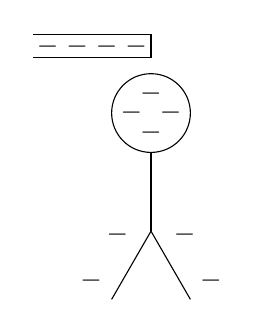
\begin{tikzpicture}[scale=0.5]
                \draw (-3,2) -- (0,2) -- (0,1.4) -- (-3,1.4);
                \foreach \j in {-2.625,-1.875,-1.125,-0.375} {
                    \node[anchor=center] at (\j,1.7cm) {$-$};
                }
                \draw (0,0) circle (1cm);
                \foreach \i in {0,90,180,270} {
                    \node[anchor=center] at (\i:0.5cm) {$-$};
                }
                \draw (0,-1) -- (0,-3);
                \draw (0,-3) -- ++(240:2cm)
                    node[anchor=south east,pos=0.33] {$-$}
                    node[anchor=south east,pos=1.00] {$-$};
                \draw (0,-3) -- ++(300:2cm)
                    node[anchor=south west,pos=0.33] {$-$}
                    node[anchor=south west,pos=1.00] {$-$};
            \end{tikzpicture}
        }
        \wrongchoice{
            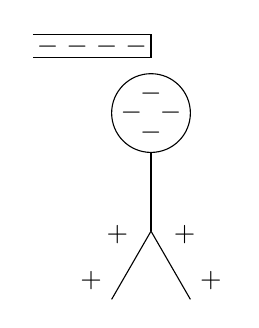
\begin{tikzpicture}[scale=0.5]
                \draw (-3,2) -- (0,2) -- (0,1.4) -- (-3,1.4);
                \foreach \j in {-2.625,-1.875,-1.125,-0.375} {
                    \node[anchor=center] at (\j,1.7cm) {$-$};
                }
                \draw (0,0) circle (1cm);
                \foreach \i in {0,90,180,270} {
                    \node[anchor=center] at (\i:0.5cm) {$-$};
                }
                \draw (0,-1) -- (0,-3);
                \draw (0,-3) -- ++(240:2cm)
                    node[anchor=south east,pos=0.33] {$+$}
                    node[anchor=south east,pos=1.00] {$+$};
                \draw (0,-3) -- ++(300:2cm)
                    node[anchor=south west,pos=0.33] {$+$}
                    node[anchor=south west,pos=1.00] {$+$};
            \end{tikzpicture}
        }
        \correctchoice{
            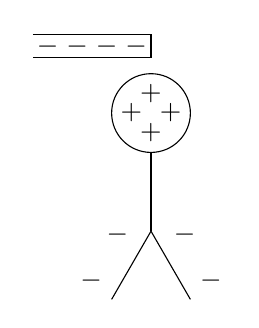
\begin{tikzpicture}[scale=0.5]
                \draw (-3,2) -- (0,2) -- (0,1.4) -- (-3,1.4);
                \foreach \j in {-2.625,-1.875,-1.125,-0.375} {
                    \node[anchor=center] at (\j,1.7cm) {$-$};
                }
                \draw (0,0) circle (1cm);
                \foreach \i in {0,90,180,270} {
                    \node[anchor=center] at (\i:0.5cm) {$+$};
                }
                \draw (0,-1) -- (0,-3);
                \draw (0,-3) -- ++(240:2cm)
                    node[anchor=south east,pos=0.33] {$-$}
                    node[anchor=south east,pos=1.00] {$-$};
                \draw (0,-3) -- ++(300:2cm)
                    node[anchor=south west,pos=0.33] {$-$}
                    node[anchor=south west,pos=1.00] {$-$};
            \end{tikzpicture}
        }
        \wrongchoice{
            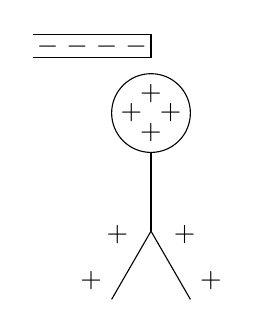
\begin{tikzpicture}[scale=0.5]
                \draw (-3,2) -- (0,2) -- (0,1.4) -- (-3,1.4);
                \foreach \j in {-2.625,-1.875,-1.125,-0.375} {
                    \node[anchor=center] at (\j,1.7cm) {$-$};
                }
                \draw (0,0) circle (1cm);
                \foreach \i in {0,90,180,270} {
                    \node[anchor=center] at (\i:0.5cm) {$+$};
                }
                \draw (0,-1) -- (0,-3);
                \draw (0,-3) -- ++(240:2cm)
                    node[anchor=south east,pos=0.33] {$+$}
                    node[anchor=south east,pos=1.00] {$+$};
                \draw (0,-3) -- ++(300:2cm)
                    node[anchor=south west,pos=0.33] {$+$}
                    node[anchor=south west,pos=1.00] {$+$};
            \end{tikzpicture}
        }
    \end{choices}
    \end{multicols}
\end{question}
}

\element{cpo-mc}{
\begin{question}{cpo-ch15-q11}
    A rod and a piece of cloth are rubbed together.
    If the rod acquires a charge of \SI[retain-explicit-plus]{+1e-6}{\coulomb},
        the cloth acquires a charge of:
    \begin{multicols}{2}
    \begin{choices}
        \wrongchoice{\SI{0e0}{\coulomb}}
        \wrongchoice{\SI[retain-explicit-plus]{+1e-6}{\coulomb}}
      \correctchoice{\SI[retain-explicit-plus]{-1e-6}{\coulomb}}
        \wrongchoice{\SI[retain-explicit-plus]{+1e+6}{\coulomb}}
    \end{choices}
    \end{multicols}
\end{question}
}

\element{cpo-mc}{
\begin{question}{cpo-ch15-q12}
    An electrically neutral object can be attracted by a positively charged object because:
    \begin{choices}
        \wrongchoice{like charges repel each other.}
      \correctchoice{the charges on a neutral object can be redistributed.}
        \wrongchoice{the neutral object becomes charged by friction.}
        \wrongchoice{the neg charge in a system varies.}
    \end{choices}
\end{question}
}

\element{cpo-mc}{
\begin{questionmult}{ch15-Q13}
    Two charged spheres are placed \SI{9}{\meter} apart,
        as shown below.
    \begin{center}
    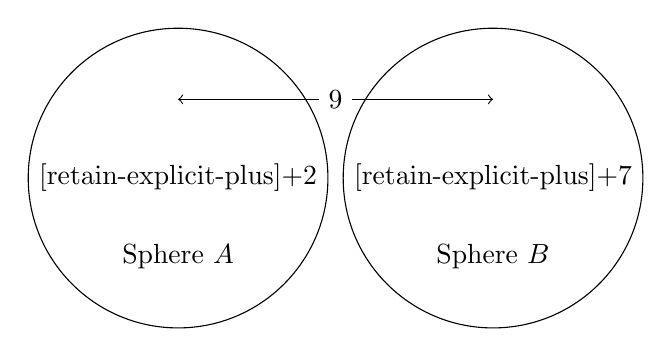
\begin{tikzpicture}
        \node[draw,circle,minimum size=1.00cm] (A) at (-2,0) {\SI[retain-explicit-plus]{+2}{\coulomb}};
        \node[draw,circle,minimum size=1.00cm] (B) at (+2,0) {\SI[retain-explicit-plus]{+7}{\coulomb}};
        \node[below of=A] at (A) {Sphere $A$};
        \node[below of=B] at (B) {Sphere $B$};
        \draw[<->] (-2,1) -- (2,1) node[fill=white,pos=0.5] {\SI{9}{\meter}};
    \end{tikzpicture}
    \end{center}
    Determine the electric force exerted on sphere $A$?
    \begin{multicols}{2}
    \begin{choices}
        \wrongchoice{\SI{9e9}{\newton}}
        \wrongchoice{\SI{1.3e11}{\newton}}
        \wrongchoice{\SI{1.4e10}{\newton}}
      \correctchoice{\SI{1.6e9}{\newton}}
    \end{choices}
    \end{multicols}
\end{questionmult}
}

\element{cpo-mc}{
\begin{question}{cpo-ch15-q14}
    As the distance between two positively charged objects increases, the force between then:
    \begin{choices}
        \wrongchoice{increases.}
      \correctchoice{decreases.}
        \wrongchoice{cannot be determined.}
        \wrongchoice{remains the same.}
    \end{choices}
\end{question}
}

\element{cpo-mc}{
\begin{question}{cpo-ch15-q15}
    The electric force between a \SI{5}{\coulomb} charge and a \SI{1}{\coulomb} charge \SI{9 000}{\meter} apart is:
    \begin{multicols}{2}
    \begin{choices}
        \wrongchoice{\SI{5 000 000}{\newton}}
        \wrongchoice{\SI{666}{\newton}}
      \correctchoice{\SI{556}{\newton}}
        \wrongchoice{\SI{0.000 556}{\newton}}
    \end{choices}
    \end{multicols}
\end{question}
}

\element{cpo-mc}{
\begin{question}{cpo-ch15-q16}
    If the distance between two charges is reduced by half,
        the electric force between then:
    \begin{choices}
        \wrongchoice{decreases by \num{1/2}.}
        \wrongchoice{decreases by \num{1/4}.}
        \wrongchoice{increases by \num{2} times.}
      \correctchoice{increases by \num{4} times.}
    \end{choices}
\end{question}
}

\element{cpo-mc}{
\begin{question}{cpo-ch15-q17}
    Two points charges attract each other with a force of \SI{8.0e-5}{\newton}.
    If the distance between the charges is doubled,
        the force of attraction will become:
    \begin{multicols}{2}
    \begin{choices}
        \wrongchoice{\SI{16e-5}{\newton}}
      \correctchoice{\SI{2.0e-5}{\newton}}
        \wrongchoice{\SI{64e-5}{\newton}}
        \wrongchoice{\SI{4.0e-5}{\newton}}
    \end{choices}
    \end{multicols}
\end{question}
}

\element{cpo-mc}{
\begin{question}{cpo-ch15-q18}
    Suppose you rub an inflated party balloon on a carpet,
        hold the balloon next to a wall, and discover that it ``sticks'' to the wall.
    Why did the balloon stick to the wall?
    \begin{choices}
        \wrongchoice{The total charge on the balloon and wall becomes zero, so attraction between the two can occur.}
        \wrongchoice{Like charges on the balloon and wall cause an attraction between the two.}
        \wrongchoice{Balloons contain a special ``atomic glue'' that holds them to cling to other objects.}
      \correctchoice{Excess charge builds up on the balloon and electrostatic forces allow the balloon and the wall to be attracted to one another.}
    \end{choices}
\end{question}
}

\element{cpo-mc}{
\begin{question}{cpo-ch15-q19}
    An electric current in a metal consists of moving:
    \begin{multicols}{2}
    \begin{choices}
        \wrongchoice{nuclei.}
        \wrongchoice{protons.}
        \wrongchoice{neutrons.}
      \correctchoice{electrons.}
    \end{choices}
    \end{multicols}
\end{question}
}

\element{cpo-mc}{
\begin{question}{cpo-ch15-q20}
    Because of Ben Franklin's work, the direction of current
        in an electrical circuit is defined as going from:
    \begin{choices}
        \wrongchoice{positive to negative.}
      \correctchoice{negative to positive.}
        \wrongchoice{positive to positive.}
        \wrongchoice{negative to negative.}
    \end{choices}
\end{question}
}

\element{cpo-mc}{
\begin{question}{cpo-ch15-q21}
    Almost all of the electrons flowing through a battery circuit come from atoms:
    \begin{choices}
      \correctchoice{in the wire conductor.}
        \wrongchoice{in the circuit components.}
        \wrongchoice{involved in chemical reactions at the battery's negative terminal.}
        \wrongchoice{involved in chemical reactions at the battery's positive terminal.}
    \end{choices}
\end{question}
}

\element{cpo-mc}{
\begin{question}{cpo-ch15-q22}
    The electrons in an insulator are best described as:
    \begin{choices}
        \wrongchoice{free to move.}
      \correctchoice{fixed in place.}
        \wrongchoice{flowing charges.}
        \wrongchoice{a potential difference.}
    \end{choices}
\end{question}
}

%\element{cpo-mc}{
%\begin{question}{cpo-ch15-q23}
%    The electric field around two positive charges looks most like:
%    \begin{multicols}{2}
%    \begin{choices}[o]
%        %% NOTE: TODO: needs field line diagrams
%        %\wrongchoice{
%        %    \begin{tikzpicture}
%        %    \end{tikzpicture}
%        %}
%    \end{choices}
%    \end{multicols}
%\end{question}
%}

\element{cpo-mc}{
\begin{question}{cpo-ch15-q24}
    A capacitor can be charged by:
    \begin{multicols}{2}
    \begin{choices}
        \wrongchoice{A resistor}
      \correctchoice{A battery}
        \wrongchoice{wires}
        \wrongchoice{an ammeter}
    \end{choices}
    \end{multicols}
\end{question}
}

\element{cpo-mc}{
\begin{question}{cpo-ch15-q25}
    Capacitance is measured in units of:
    \begin{multicols}{2}
    \begin{choices}
      \correctchoice{farad (\si{\farad})}
        \wrongchoice{volt (\si{\volt})}
        \wrongchoice{ohm (\si{\ohm})}
        \wrongchoice{joule (\si{\joule})}
    \end{choices}
    \end{multicols}
\end{question}
}

\element{cpo-mc}{
\begin{question}{cpo-ch15-q26}
    A capacitor is a device that:
    \begin{choices}
        \wrongchoice{charges electrons.}
        \wrongchoice{charges protons.}
      \correctchoice{stores electrical energy.}
        \wrongchoice{stores chemical energy.}
    \end{choices}
\end{question}
}

\element{cpo-mc}{
\begin{questionmult}{ch15-Q27}
    When a capacitor is discharged:
    \begin{choices}
      \correctchoice{it creates a current until all its stored energy has been converted.}
      \correctchoice{the current it creates decreases over time.}
      \correctchoice{electrons move from the negative plate to the positive plate until both plates are neutral.}
    \end{choices}
\end{questionmult}
}

\element{cpo-mc}{
\begin{question}{cpo-ch15-q28}
    Capacitance is the:
    \begin{choices}
      \correctchoice{ability of a capacitor to store charge.}
        \wrongchoice{ability of a capacitor to store resistance.}
        \wrongchoice{buildup of electric charge on an object.}
        \wrongchoice{flow of electric charge.}
    \end{choices}
\end{question}
}

\element{cpo-mc}{
\begin{question}{cpo-ch15-q29}
    All of the following will increase the capacitance of a parallel plate capacitor \emph{except}:
    \begin{choices}
        \wrongchoice{increasing the size of the capacitor's plates.}
      \correctchoice{increasing the voltage of the battery that charges it.}
        \wrongchoice{using a material that provides better insulation between the plates.}
        \wrongchoice{decreasing the distance between the plates.}
    \end{choices}
\end{question}
}


\endinput



